\documentclass{beamer}
\usetheme{Madrid}
\usecolortheme{beaver} % Academic Red/Grey theme

\usepackage[utf8]{inputenc}
\usepackage{graphicx}
\usepackage{amsmath}
\usepackage{tikz}
\usetikzlibrary{arrows, positioning, calc}

% Presentation Info
\title[Hydrokinetic Energy]{Hydrokinetic Energy Conversion Systems}
\subtitle{Analysis, Design, and Implementation Strategies}
\author[Group 10]{Hamidreza Khalaj Zahrari \and Muhammet Yağcıoğlu}
\institute[IZTECH]{
    \textbf{Izmir Institute of Technology} \\
    Civil Engineering Department
}
\date{January 5, 2026}

\begin{document}

% Slide 1: Title
\begin{frame}
    \titlepage
\end{frame}

% Slide 2: Introduction
\begin{frame}{Introduction to Hydrokinetic Energy}
    \begin{columns}
        \begin{column}{0.6\textwidth}
            \begin{itemize}
                \item \textbf{Definition:} A renewable energy technology that converts the kinetic energy of moving water (rivers, tides, ocean currents) into electricity without the need for impoundments (dams).
                \item \textbf{Core Concept:} Analogous to wind turbines but operating in a fluid medium $\approx 830$ times denser than air.
                \item \textbf{Significance:} Offers a baseload renewable energy source with minimal civil infrastructure requirements.
            \end{itemize}
        \end{column}
        \begin{column}{0.4\textwidth}
            \centering
            % Simple TikZ Turbine Icon
            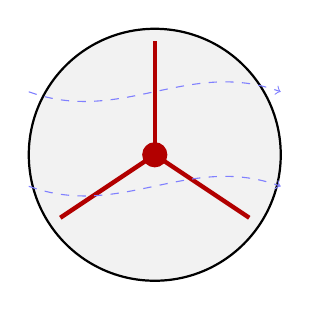
\begin{tikzpicture}[scale=0.8]
                \draw[thick, fill=gray!10] (0,0) circle (2);
                \draw[ultra thick, red!70!black] (0,0) -- (0,1.8);
                \draw[ultra thick, red!70!black] (0,0) -- (1.5,-1);
                \draw[ultra thick, red!70!black] (0,0) -- (-1.5,-1);
                \fill[red!70!black] (0,0) circle (0.2);
                \draw[blue!50, dashed, ->] (-2,1) to[out=-20,in=160] (2,1);
                \draw[blue!50, dashed, ->] (-2,-0.5) to[out=-20,in=160] (2,-0.5);
            \end{tikzpicture}
        \end{column}
    \end{columns}
\end{frame}

% Slide 3: Working Principle
\begin{frame}{Working Principle \& System Architecture}
    \begin{columns}
        \begin{column}{0.5\textwidth}
            The system operates on the principle of hydrodynamic lift and drag.
            \begin{block}{Energy Conversion Equation}
                \begin{equation}
                    P = \frac{1}{2} \rho A v^3 C_p \eta
                \end{equation}
                \footnotesize{Where $\eta$ represents the mechanical/electrical efficiency.}
            \end{block}
            \begin{itemize}
                \item \textbf{Rotor:} Captures kinetic energy.
                \item \textbf{Powertrain:} Increases rotational speed.
                \item \textbf{Generator:} Converts to electricity.
            \end{itemize}
        \end{column}
        \begin{column}{0.5\textwidth}
            \centering
            \includegraphics[width=\textwidth, height=0.6\textheight, keepaspectratio]{working.png}
            \vspace{0.2cm}
            \textit{\footnotesize Figure 1: Schematic representation.}
        \end{column}
    \end{columns}
\end{frame}

% Slide 4: Hydrodynamic Analysis (TikZ)
\begin{frame}{Hydrodynamic Analysis: Velocity Triangles}
    Understanding the flow interaction at the blade section is critical for efficiency ($C_p$).
    
    \begin{center}
        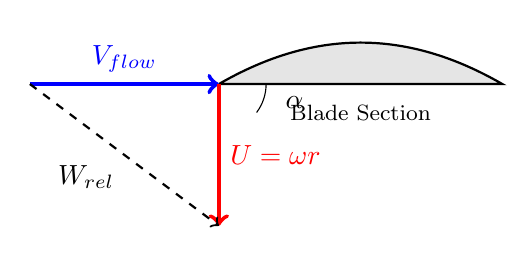
\begin{tikzpicture}[scale=1.2]
            % Blade Section
            \draw[thick, fill=gray!20] (0,0) to[out=30,in=150] (3,0) to[out=180,in=0] (0,0);
            \node at (1.5, -0.3) {\footnotesize Blade Section};
            
            % Vectors
            \draw[->, ultra thick, blue] (-2,0) -- (0,0) node[midway, above] {$V_{flow}$};
            \draw[->, ultra thick, red] (0,0) -- (0,-1.5) node[midway, right] {$U = \omega r$};
            \draw[->, thick, dashed] (-2,0) -- (0,-1.5) node[midway, below left] {$W_{rel}$};
            
            % Angle
            \draw (0.5,0) arc (0:-37:0.5);
            \node at (0.8,-0.2) {$\alpha$};
        \end{tikzpicture}
    \end{center}
    
    \begin{itemize}
        \item $V_{flow}$: Absolute velocity of the water current.
        \item $U$: Tangential velocity of the blade ($\omega \cdot r$).
        \item $W_{rel}$: Relative velocity seen by the blade.
        \item $\alpha$: Angle of attack, determining Lift ($L$) and Drag ($D$) forces.
    \end{itemize}
\end{frame}

% Slide 5: Comparison
\begin{frame}{Comparative Analysis}
    \begin{table}
        \begin{tabular}{|l|l|l|}
            \hline
            \textbf{Parameter} & \textbf{Conventional Hydro} & \textbf{Hydrokinetic Systems} \\
            \hline
            \textbf{Primary Energy} & Potential Head ($H$) & Kinetic Velocity ($v$) \\
            \hline
            \textbf{Civil Works} & Extensive (Dams) & Minimal (Anchors) \\
            \hline
            \textbf{Environmental} & High Impact & Low Impact \\
            \hline
            \textbf{Scalability} & Site-specific & Modular \\
            \hline
        \end{tabular}
    \end{table}
\end{frame}

% Slide 6: Turkey Context
\begin{frame}{Implementation Potential in Turkey}
    \begin{columns}
        \begin{column}{0.5\textwidth}
            \begin{block}{The Turkish Straits}
                The Bosphorus and Dardanelles represent a massive energy corridor with continuous two-way currents.
            \end{block}
            \begin{block}{Irrigation Networks}
                DSİ channels in the GAP region offer controlled, debris-free flow environments.
            \end{block}
        \end{column}
        \begin{column}{0.5\textwidth}
            \textbf{Current Initiatives}
            \begin{itemize}
                \item \textbf{Mavi İda Enerji:} "M30" Turbine (Çanakkale).
                \item \textbf{TOBB ETÜ:} Micro-hydro and in-pipe systems.
                \item \textbf{Academic Research:} IZTECH, ITU, and METU are leading CFD and experimental studies.
            \end{itemize}
        \end{column}
    \end{columns}
\end{frame}

% Slide 7: Civil Engineering Challenges
\begin{frame}{Civil Engineering Challenges}
    \begin{itemize}
        \item \textbf{Foundation Systems:}
        \begin{itemize}
            \item \textit{Gravity Based Structures (GBS):} Rely on mass.
            \item \textit{Monopiles:} Driven into the seabed.
        \end{itemize}
        \item \textbf{Structural Dynamics:} Fatigue analysis of blades.
        \item \textbf{Scour Protection:} Preventing seabed erosion.
    \end{itemize}
    
    \begin{alertblock}{Critical Design Factor}
        The cubic relationship ($P \propto v^3$) implies that structural loads increase drastically with velocity. Safety factors must account for extreme flow events.
    \end{alertblock}
\end{frame}

% Slide 8: Conclusion
\begin{frame}{Conclusion}
    \begin{itemize}
        \item Hydrokinetic energy represents a paradigm shift from "static" to "dynamic" hydropower.
        \item Aligns with sustainable development goals by minimizing civil footprint.
        \item \textbf{Role of Civil Engineers:} Essential for ensuring the structural integrity, foundation stability, and environmental compatibility.
    \end{itemize}
    \vspace{1cm}
    \centering
    \textcolor{darkred}{\textbf{\Large Thank You}}
\end{frame}

\end{document}
